\documentclass[]{tufte-handout}

% ams
\usepackage{amssymb,amsmath}

\usepackage{ifxetex,ifluatex}
\usepackage{fixltx2e} % provides \textsubscript
\ifnum 0\ifxetex 1\fi\ifluatex 1\fi=0 % if pdftex
  \usepackage[T1]{fontenc}
  \usepackage[utf8]{inputenc}
\else % if luatex or xelatex
  \makeatletter
  \@ifpackageloaded{fontspec}{}{\usepackage{fontspec}}
  \makeatother
  \defaultfontfeatures{Ligatures=TeX,Scale=MatchLowercase}
  \makeatletter
  \@ifpackageloaded{soul}{
     \renewcommand\allcapsspacing[1]{{\addfontfeature{LetterSpace=15}#1}}
     \renewcommand\smallcapsspacing[1]{{\addfontfeature{LetterSpace=10}#1}}
   }{}
  \makeatother
\fi

% graphix
\usepackage{graphicx}
\setkeys{Gin}{width=\linewidth,totalheight=\textheight,keepaspectratio}

% booktabs
\usepackage{booktabs}

% url
\usepackage{url}

% hyperref
\usepackage{hyperref}

% units.
\usepackage{units}


\setcounter{secnumdepth}{-1}

% citations
\usepackage{natbib}
\bibliographystyle{plainnat}

% pandoc syntax highlighting

% longtable

% multiplecol
\usepackage{multicol}

% strikeout
\usepackage[normalem]{ulem}

% morefloats
\usepackage{morefloats}


% tightlist macro required by pandoc >= 1.14
\providecommand{\tightlist}{%
  \setlength{\itemsep}{0pt}\setlength{\parskip}{0pt}}

% title / author / date

%\usepackage[top=1in, bottom=1in, left=1in, right=1in]{geometry}
%\geometry{top=1in, bottom=1in, left=1in, right=1in}
\geometry{
  %left=24.8mm, % left margin
  %textwidth=100mm, % main text block
  %marginparsep=8.2mm, % gutter between main text block and margin notes
  %marginparwidth=49.4mm, % width of margin notes
  bottom=1in
}

\usepackage{setspace}
\usepackage{graphicx}
\usepackage{subfig}
\usepackage[UKenglish]{babel,isodate}% http://ctan.org/pkg/babel
\usepackage[nottoc]{tocbibind}
\setcounter{tocdepth}{4}
\setcounter{secnumdepth}{-2}

\usepackage{amsmath,amssymb} %allows use of maths symbols

\makeatletter % this renews the paragraph setting to behave more like a 'subsubsubsection'
\renewcommand\paragraph{\@startsection{paragraph}{4}{\z@}%
            {-2.5ex\@plus -1ex \@minus -.25ex}%
            {1.25ex \@plus .25ex}%
            {\normalfont\normalsize\bfseries}}
\makeatother

\usepackage{fancyhdr}
\pagestyle{fancyplain}
\usepackage{lastpage}
\fancyhf[HRO]{Ongoing emergencies: contributions \& pledges}
\fancyhf[HLO]{}
\fancyhf[HRE]{Ongoing emergencies: contributions \& pledges}
%\fancyfoot[C]{\sffamily\fontsize{9pt}{9pt}\selectfont\thepage}
\fancyfoot[C]{\fontsize{9pt}{9pt}\thepage}

\raggedbottom
\setlength\parindent{0pt} % sets indent to zero
\setlength{\parskip}{2mm}

\usepackage{hyperref}
\usepackage[usenames,dvipsnames]{xcolor}
\hypersetup{
    colorlinks,
    citecolor=black,
    filecolor=black,
    linkcolor=BlueViolet,
    urlcolor=BlueViolet
}
\usepackage{colortbl}
\definecolor{whoblue}{rgb}{0.00, 0.60, 0.80}

\usepackage[utf8]{inputenc}
\usepackage[T1]{fontenc}
%\usepackage{soul} %for highlighting text [\hl{TEXT}]

%\IfFileExists{bergamo.sty}{\usepackage[osf]{bergamo}}{}% Bembo
%\IfFileExists{chantill.sty}{\usepackage{chantill}}{}% Gill Sans
%\IfFileExists{opensans.sty}{\usepackage[default,scale=0.95]{opensans}}{}
%\usepackage[default,scale=0.95]{opensans}
%\usepackage{fontspec} % For use with xelatex, not pdflatex!!
%\setmainfont{Arial}

\usepackage{booktabs}
\usepackage{tabularx}
\usepackage{multirow}
\usepackage{pdflscape}
\usepackage{pdfpages} %for inserting PDFs into document
\usepackage{rotating}
\usepackage{longtable}

%\usepackage[labelfont=bf]{caption} % package clash for some reason - use below 2 commands instead!!
\usepackage{caption}
\captionsetup{labelfont=bf}

\usepackage{float}
\floatplacement{figure}{H}

\makeatletter
\newenvironment{keeppage}{\let\thispagestyle=\@gobble}{}
\makeatother

\newcommand{\HRule}{\rule{\linewidth}{0.5mm}}

\begin{document}



%\newgeometry{margin=1in}
\begin{titlepage}

\hspace*{-1cm}\begin{minipage}[t][0.1\textheight]{5cm}
\textcolor{whoblue!15}{\rule{5cm}{0.1\textheight}}
\end{minipage}
\hspace*{1cm}\begin{minipage}[t]{11.3cm}
\textcolor{whoblue}{\rule{11.3cm}{0.5mm}}
\end{minipage}

\hspace*{-1cm}\begin{minipage}[t][0.1\textheight]{5cm}
\vspace{0pt}

\includegraphics[height=0.1\textheight]{figure/logo_paho.png}\\[0.55cm]
\textcolor{whoblue!15}{\rule{5cm}{0.1\textheight}}
\end{minipage}
\hspace*{1cm}\begin{minipage}[t][0.2\textheight]{11.3cm}{}
\vspace{0pt}
\begin{flushright}
\begin{spacing}{2.0}
%{\Huge\bfseries Grade 3 and Grade 2 emergencies, and ERM priority countries}
%{\Huge \textbf{Grade 3 and Grade 2 emergencies, and ERM priority countries}}
% \textbf{Grade 3 and Grade 2 emergencies, and ERM priority countries}
{\huge \textbf{Ouragan Matthew réponse, Département de la Grand’ Anse, Haiti}}
\end{spacing}
\end{flushright}
\end{minipage}

\hspace*{-1cm}\begin{minipage}[0.1\textheight]{5cm}
\vspace{0pt}

\includegraphics[height=0.1\textheight]{figure/logo_who}
\end{minipage}
\hspace*{1cm}\begin{minipage}{11.3cm}
\vspace{0pt}
\begin{flushright}
\begin{spacing}{1.0}
{\LARGE Rapport sur le renforcement de la surveillance épidémiologique et gestion des données}
%Contributions and Firm Pledges
\end{spacing}
\end{flushright}
\end{minipage}

\hspace*{-1cm}\begin{minipage}[t]{5cm}
\vspace{0pt}
\textcolor{whoblue!15}{\rule{5cm}{0.577\textheight}}
\end{minipage}
\hspace*{1cm}\begin{minipage}[t]{11.3cm}
\vspace{0pt}
\textcolor{whoblue}{\rule{11.3cm}{0.5mm}}\\[0.465\textheight]
\begin{flushright}
{\Large \bf{Jonathan Polonsky}}\\
{\Large Epidemiologist}\\
{\Large WHO Emergencies Programme}\\[0.5cm]
\cleanlookdateon \textsc{\large \today}
\end{flushright}
\end{minipage}

\end{titlepage}
%\restoregeometry


\section{Background}\label{background}

\newthought{On 4 October, Hurricane Matthew} violently struck Haiti and
resulted in the country's largest humanitarian emergency since the 2010
earthquake. It caused extensive flooding and mudslides, damage to road
infrastructure and buildings, as well as electricity and water
shortages. The latest figures from the governmental Directorate of Civil
Protection (DPC) of Haiti have so far confirmed 546 deaths and 438
injured as a result of the hurricane.

Humanitarian needs are said to include access to a sufficient supply of
quality water, education, shelter, child protection, health, and
nutrition. Of the 1.4 million people who need humanitarian assistance,
more than 40 per cent are children who are mainly in the Grand'Anse
(DSGA) and Sud Departments

In this context, I was deployed for just over 2 weeks as a field
epidemiologist to Jeremie, the departmental capital of DSGA, to analyse
the situation and provide support to the PAHO country office in
assisting the Ministère de la Santé Publique et de la Population (MSPP)
in re-establishing/strengthening epidemic-prone disease surveillance in
the affected areas.

\section{Data collection, management, analysis \&
reporting}\label{data-collection-management-analysis-reporting}

\newthought{An initial assessment of} the ongoing data collection,
management and reporting system in place for suspected cholera
highlighted potential areas for rapid gains. The processes that feed
into these components are described below:

\subsection{Data collection \&
management}\label{data-collection-management}

\newthought{Every day, the PAHO field epiemiologist} or the MSPP
departmental epidemiologist telephone each Cholera Treatment Centre/Unit
(CTC/UTC) to get aggregated information read to them: \# cases seen; \#
cases hospitalised; \# institutional deaths; \# community deaths. All of
these are reported for two age groups: \textless{}5 and 5+ years. These
phone calls were made twice per day - the first to report overnight
changes, and a follow up call made later in the day to find out any
further changes during the day.

The data are entered into an excel workbook. With each new day, eight
new columns must be added (representing the four variables and two age
groups for each). This workbook has data going back to 1st Jan 2012, and
is now very wide (\textgreater{} 14,500 columns) and heavy
(\textasciitilde{} 40MB). The workbook is (sensibly) protected, but this
means that analysing the data is cumbersome - the epidemiologist in
place was double entering the data each day, once in this workbook and
once in a separate workbook covering just the days since the hurricane.

\subsection{Analysis \& reporting}\label{analysis-reporting}

\newthought{In order to analyse} the data since hurricane Matthew, some
figures had been created within this second, unprotected excel workbook,
and each day these could be updated with the new data. However, because
there were a large number of figures (some for overall analyses, and one
each for the 17 operational CTCs), this was yet another cumbersome
process as the data range for each needed to be manually updated.

These updated graphs were subsequently copied and pasted into a word
document, along with a table of the updated data, and this was
circulated each day to relevant partners.

\subsection{Changes made}\label{changes-made}

\newthought{The following changes were} implemented:

\begin{itemize}
\tightlist
\item
  Lighter reporting schedule

  \begin{itemize}
  \tightlist
  \item
    only one contact made per day to each CTC to reduce burden on both
    CTC staff and epidemiologist

    \begin{itemize}
    \tightlist
    \item
      this should only cover the previous day in completeness
    \end{itemize}
  \item
    a brief (1-page) report of the previous day with a table of new
    cases by commune \& CTC
  \item
    a longer in-depth report issued once per week covering the previous
    epidemic week in completeness (each epidemic week runs from Sunday
    to Saturday)

    \begin{itemize}
    \tightlist
    \item
      broader trends should be analysed on a weekly, not daily basis
    \end{itemize}
  \end{itemize}
\item
  Automated analysis \& reporting

  \begin{itemize}
  \tightlist
  \item
    As the weekly report has a standardised format, and only needs to
    take into account updates to the dataset each week, the analysis and
    reporting were perfect candidates for automation. I wrote a script
    in the \texttt{R\ statistical\ language}\footnote{\href{https://www.r-project.org/}{The
      R Project for Statistical Computing}} to read in the data, analyse
    it, generate various tables, figures and maps, and output these into
    a standardised PDF report. The report takes \textasciitilde{}20
    seconds to generate, rather than \textgreater{}1 hour as was
    previously the case.
  \item
    This report, approved by MSPP at the departmental level, is shared
    with MSPP before the weekly surveillance meeting each Wednesday, and
    the responsibility of sharing the report is handed over to MSPP, as
    the data are of course owned by the country, not PAHO.
  \end{itemize}
\end{itemize}

\section{Epidemiological context}\label{epidemiological-context}

\newthought{Extracts of the automated} report are included in this
report to demonstrate the outputs and to describe the current
epidemiological situation regarding suspected cholera cases in the
Département de la Grand' Anse.

\begin{figure*}
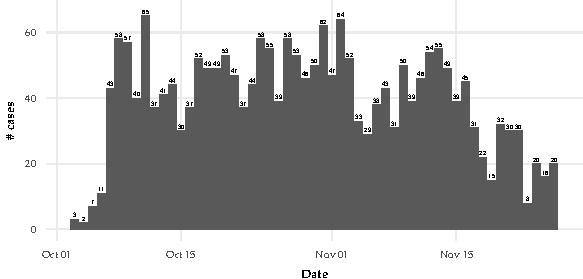
\includegraphics{rapport_final_files/figure-latex/epicurve_all-1} \caption[Tendance des cas de diarrhées aigues, 03 Oct 2016 - 26 Nov 2016 Grand’Anse (données partielles)]{Tendance des cas de diarrhées aigues, 03 Oct 2016 - 26 Nov 2016 Grand’Anse (données partielles).}\label{fig:epicurve_all}
\end{figure*}

Following a rapid increase in cases of suspected cholera following
Hurricane Matthew, from fewer than 10 cases per day to a mean of around
50 cases per day until the middle of November, after which time the
cases steadily declined to around 20 cases per day during epiweek 47
(Figure \ref{fig:epicurve_all}).

\clearpage

\begin{fullwidth}
\makeatletter\setlength\hsize{\@tufte@fullwidth}\setlength\linewidth{\@tufte@fullwidth}\let\caption\@tufte@orig@caption\makeatother
\footnotesize
\begin{longtable}{llrrrr}
\caption{Répartition des cas de diarrhées aigues par CTC/UTC, 03 Oct 2016 - 26 Nov 2016 Grand’Anse (données partielles).} \\ 
  \toprule
Commune & UTC/CTC & Cas (\%) & Décès inst. (\%) & Décès comm. (\%) & Total décès \\ 
  \midrule
Abricots & Bontemps & 5 (0.2) & 0 (0) & 0 (0) & 0 \\ 
   \rowcolor{whoblue!15}Abricots & SSPE des Abrcots & 67 (3.1) & 3 (4.8) & 0 (0) & 3 \\ 
  Anse-d'Hainault & HCR Anse d'Hainault & 447 (20.6) & 10 (15.9) & 1 (11.1) & 11 \\ 
   \rowcolor{whoblue!15}Anse-d'Hainault & UTC Sicard & 1 (0) & 0 (0) & 0 (0) & 0 \\ 
  Beaumont & Citymed & 11 (0.5) & 0 (0) & 0 (0) & 0 \\ 
   \rowcolor{whoblue!15}Bonbon & Bonbon & 9 (0.4) & 0 (0) & 2 (22.2) & 2 \\ 
  Chambellan & Centre de santé de Chambellan & 134 (6.2) & 3 (4.8) & 1 (11.1) & 4 \\ 
   \rowcolor{whoblue!15}Dame-Marie & UTC Dame-Marie & 109 (5) & 7 (11.1) & 0 (0) & 7 \\ 
  Jeremie & Gond Ayer & 55 (2.5) & 9 (14.3) & 0 (0) & 9 \\ 
   \rowcolor{whoblue!15}Jeremie & Hôpital St-Antoine & 275 (12.7) & 3 (4.8) & 0 (0) & 3 \\ 
  Jeremie & Lory & 115 (5.3) & 4 (6.3) & 0 (0) & 4 \\ 
   \rowcolor{whoblue!15}Jeremie & Marfranc & 160 (7.4) & 2 (3.2) & 0 (0) & 2 \\ 
  Jeremie & Previle & 246 (11.4) & 10 (15.9) & 0 (0) & 10 \\ 
   \rowcolor{whoblue!15}Les Irois & UTC Les Irois & 162 (7.5) & 1 (1.6) & 1 (11.1) & 2 \\ 
  Moron & UTC Moron & 323 (14.9) & 9 (14.3) & 0 (0) & 9 \\ 
   \rowcolor{whoblue!15}Pestel & UTC Pestel & 29 (1.3) & 1 (1.6) & 4 (44.4) & 5 \\ 
  Roseaux & Carrefour Charles & 17 (0.8) & 0 (0) & 0 (0) & 0 \\ 
   \rowcolor{whoblue!15}Roseaux & Grand Vincent & 0 (0) & 1 (1.6) & 0 (0) & 1 \\ 
  Total & - & 2165 (100) & 63 (-40.5) & 9 (13.3) & 72 \\ 
   \bottomrule
\label{tab_overview}
\end{longtable}
\end{fullwidth}

\clearpage

\begin{figure*}
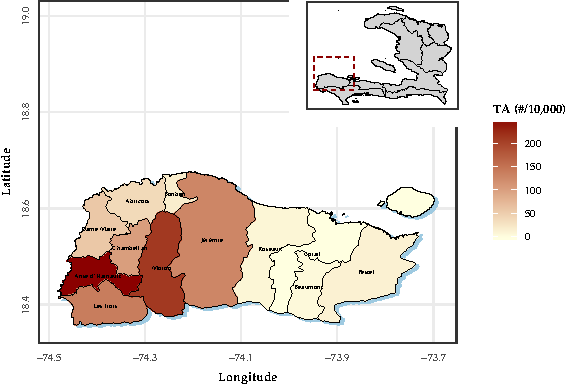
\includegraphics{rapport_final_files/figure-latex/map-1} \caption[Répresentation du taux d'attaque des cas de diarrhées aigues par 10,000 personnes, 03 Oct 2016 - 26 Nov 2016 par commune, Grand’Anse]{Répresentation du taux d'attaque des cas de diarrhées aigues par 10,000 personnes, 03 Oct 2016 - 26 Nov 2016 par commune, Grand’Anse}\label{fig:map}
\end{figure*}

The attack rate of suspected cholera follows a heterogeneous
distribution by geographic location of treatment facility, with higher
attack rates in the west of DSGA compared with those in the east (Figure
\ref{fig:map}). The highest estimated attack rates since the hurricane
have been in Anse-d'Hainhault and Moron communes (population estimations
based on 2015 census data).

\clearpage

\begin{figure*}
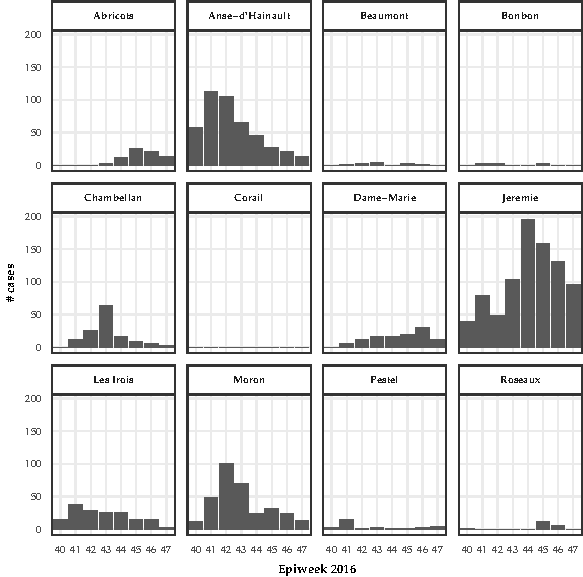
\includegraphics{rapport_final_files/figure-latex/epicurve_commune-1} \caption[Tendance des cas de diarrhées aigues, 03 Oct 2016 - 26 Nov 2016 par commune, Grand’Anse]{Tendance des cas de diarrhées aigues, 03 Oct 2016 - 26 Nov 2016 par commune, Grand’Anse}\label{fig:epicurve_commune}
\end{figure*}

The peak incidence of suspected cholera in Les Irois, Anse-d'Hainhault,
Moron and Chambellan communes occurred in epiweek 41-43, 1-3 weeks
post-hurricane, with the peak in Jérémie occurring in epiweek 44 (Figure
\ref{fig:epicurve_commune}). Abricots and Dame-Marie communes
experienced later peaks, but the absolute number of cases in these
communes was considerably lower than in the other communes mentioned
above.

\clearpage

\begin{figure*}
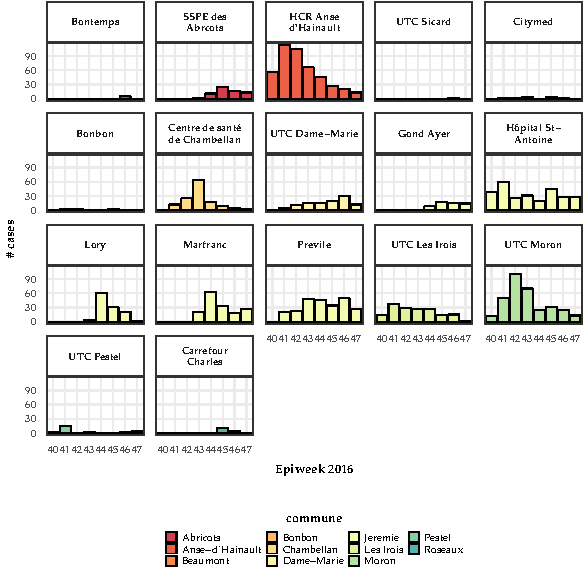
\includegraphics{rapport_final_files/figure-latex/epicurve_inst-1} \caption[Tendance des cas de diarrhées aigues, 03 Oct 2016 - 26 Nov 2016 par CTC, Grand’Anse]{Tendance des cas de diarrhées aigues, 03 Oct 2016 - 26 Nov 2016 par CTC, Grand’Anse}\label{fig:epicurve_inst}
\end{figure*}

\clearpage

\begin{figure}
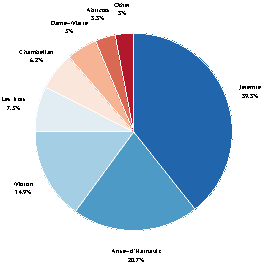
\includegraphics{rapport_final_files/figure-latex/pie-1} \caption[Répartition des cas de diarrhées aigues par commune, 03 Oct 2016 - 26 Nov 2016 Grand’Anse]{Répartition des cas de diarrhées aigues par commune, 03 Oct 2016 - 26 Nov 2016 Grand’Anse}\label{fig:pie}
\end{figure}

Approximately 40\% of cases have presented in Jérémie commune, 20\% in
Anse-d'Hainhault commune, 15\% in Moron commune, with the remaining
\textasciitilde{}25\% divided between the remaining communes (Figure
\ref{fig:pie}). Only Corail commune has not reported treating any cases
since the Hurricane, but this may reflect the heterogeneous geographic
availability of CTCs, with some patients seeking treatment in communes
other than those in which they reside.

\begin{marginfigure}
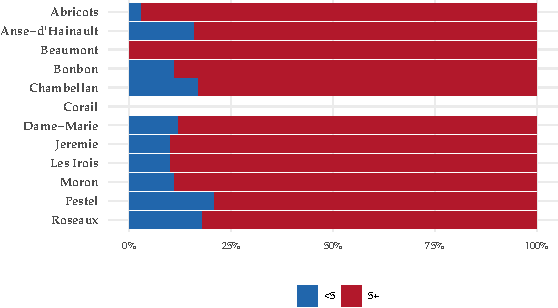
\includegraphics{rapport_final_files/figure-latex/unnamed-chunk-3-1} \caption[Répartition des cas de diarrhées aigues par tranche d'age, 03 Oct 2016 - 26 Nov 2016 par commune, Grand’Anse]{Répartition des cas de diarrhées aigues par tranche d'age, 03 Oct 2016 - 26 Nov 2016 par commune, Grand’Anse}\label{fig:unnamed-chunk-3}
\end{marginfigure}

\clearpage

\subsection{Additional sources of
data}\label{additional-sources-of-data}

\newthought{Two additional sources of information} are currently
unavailable but as they become available in the course of the coming
weeks, they should be analysed and incorporated into the regular
information products and feed into regular surveillance discussions in
DSGA:

\subsubsection{Line-listed data from health
facilities}\label{line-listed-data-from-health-facilities}

Owing to the difficulty in collecting daily data from each facility,
only aggregated data are currently collected. However, this leads to a
loss of much important granularity of the data, e.g.~provenance, sex,
treatment protocol and outcome, etc. This information is collected at
the facilities and recorded in paper registers. The Centers for Disease
Control and Prevention (CDC) are supporting MSPP and Médecins du Monde
(MDM - the NGO supporting CTCs/UTCs in DSGA) in digitizing this
information as line-lists. PAHO are providing some support to this
process by photographing the registers during field visits, and
providing these photos to MSPP/CDC for data entry. These data should be
particularly used to identify demographic and geographic risk factors
for suspected cholera transmission.

\subsubsection{Mobile clinics}\label{mobile-clinics}

On 22nd November 2016, mobile clinics were scheduled to restart their
activities having been interrupted by the hurricane and heavy rains
which had greatly hampered access to outreach communities. PAHO were
asked to review the proposed list of conditions under surveillance and
database structure in preparation for resumption of activities. Once
these data are collected and centralised in the database, they will be a
vital source of information about conditions of epidemic potential,
particularly in more inaccessible communities.

\section{Field investigations}\label{field-investigations}

\newthought{One of the roles} of the PAHO field epidemiology team is to
participate in regular field investigations. During my deployment, we
participated in 4 investigations, including alerts of clusters of
community cases and deaths (see
\protect\hyperlink{annexes}{\texttt{Annex\ 1\ \&\ 2}}), reports of
institutional deaths, and to participate in routine assessments of CTCs.
These are useful activities for a variety of reasons:

\begin{itemize}
\tightlist
\item
  strengthening the relationship between PAHO and MSPP

  \begin{itemize}
  \tightlist
  \item
    MSPP tend to rely on the availability of vehicles belonging to
    partner organisations in order to make the field visits.

    \begin{marginfigure}
    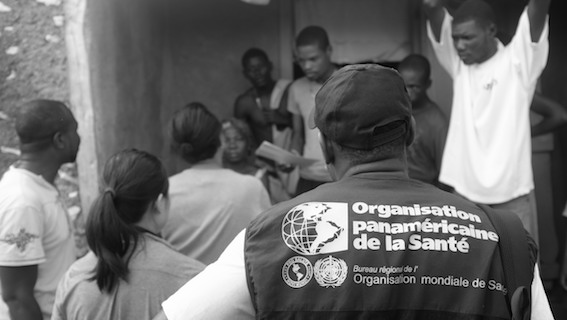
\includegraphics{figure/img1.jpg}
    \caption{Field investigation of reported community deaths conducted by joint MSPP, PAHO and CDC epidemiology team, Dame Marie commune, Grand'Anse.}
    \end{marginfigure}
  \end{itemize}
\item
  multidisciplinary visits for rationalising resources - prevents
  repeated trips to same locations and added burden to staff at CTCs
\item
  collecting and comparing data in registers with what is reported

  \begin{marginfigure}
  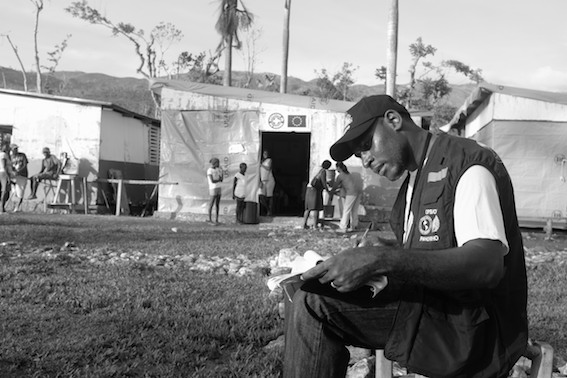
\includegraphics{figure/img2.jpg}
  \caption{PAHO epidemiologist Dr. Natael Fénelon reviewing CTC registers, Moron commune, Grand'Anse.}
  \end{marginfigure}
\end{itemize}

However, there is a sense that the approach could be more systematic and
to some extent predictable. - Under what conditions should an
investigation/field visit be launched? - what activities should be
undertaken during each visit? One important document drafted by the
cholera response team was the
\texttt{Protocole\ d’investigation\ d’une\ flambée\ de\ cholera} (see
\protect\hyperlink{annexes}{\texttt{Annex\ 3}}). Similar documents and
standard operating procedures (SOPs) that detail tasks and activities
for a variety of situations would be useful.

\clearpage

\section{Recommendations}\label{recommendations}

\begin{itemize}
\tightlist
\item
  Continue to support MSPP in field epidemiological investigations, but
  under more clearly defined SOPs.
\item
  Continue to support weekly surveillance activities through data
  compilation, analysis, reporting and coordination.
\item
  In the longer term, there is a need to transform the cholera
  surveillance system as the system currently in place is not fit for
  purpose. An improvement would be to ensure that:

  \begin{itemize}
  \tightlist
  \item
    the system is community based
  \item
    information is collected at the individual level (i.e.~line list to
    capture essential variables for analysis)
  \item
    the data entry, compilation, analysis and reporting are streamlined,
    ideally making use of the WHO-led EWARS\footnote{\href{www.ewars-project.org}{Early
      Warning Alert and Response System}} which is designed for such a
    context.
  \end{itemize}
\item
  Possible weaknesses in the surveillance system should be investigated
  and documented as an initial part of such a process in order to build
  an evidence-base for the need for modifications, perhaps through
  analyses demonstrating timeliness and completeness of reporting, and
  light-weight capture-recapture studies (as described elsewhere
  \citep{Gignoux2015, Braeye2016}) in targeted départements, to estimate
  the sensitivity of the surveillance system at 2 levels:
\item
  from the community level to the facility/CTC level (i.e.~what
  proportion of suspected cases are not detected by the surveillance
  system)
\item
  from the facility/CTC level to the departmental/central level (i.e.~do
  the data reported by the facilities accurately reflect what has been
  observed)
\item
  It is also very important to not only focus on cholera response post
  Hurricane Matthew, as there are multiple other diseases and conditions
  of great importance in the département. Some important outstanding
  questions include:

  \begin{itemize}
  \tightlist
  \item
    what has been the impact on primary health care service delivery
    (e.g.~Basic Emergency Obstetric Care)?
  \item
    malaria surveillance

    \begin{itemize}
    \tightlist
    \item
      DSGA is considered one of the areas of greatest malaria incidence
      in Haiti. Has there been an impact on malaria incidence and access
      to treatment?
    \end{itemize}
  \item
    food security/malnutrition surveillance is an important
    consideration

    \begin{itemize}
    \tightlist
    \item
      Hurricane Matthew destroyed a large proportion of the crops,
      livestock, etc in the département, and a potentially serious
      impact on food security and concomitant impact on acute
      malnutrition should be anticipated. In this case, it may be
      prudent to establish some form of community-based malnutrition
      surveillance to early-detect deteriorations in the nutritional
      status of the population, particularly among children aged under
      5. Examples and methods for such systems have been described
      elsewhere (\citet{Caleo2012}; \citet{Polonsky2013a}).
    \end{itemize}
  \end{itemize}
\end{itemize}

\clearpage

\hypertarget{annexes}{\section{Annexes}\label{annexes}}

\subsection{Annex 1 - Rapport d'investigation de cas de décès
communautaire par cholera a Desormeaux,
Grand'Anse}\label{annex-1---rapport-dinvestigation-de-cas-de-deces-communautaire-par-cholera-a-desormeaux-grandanse}

\begin{figure*}
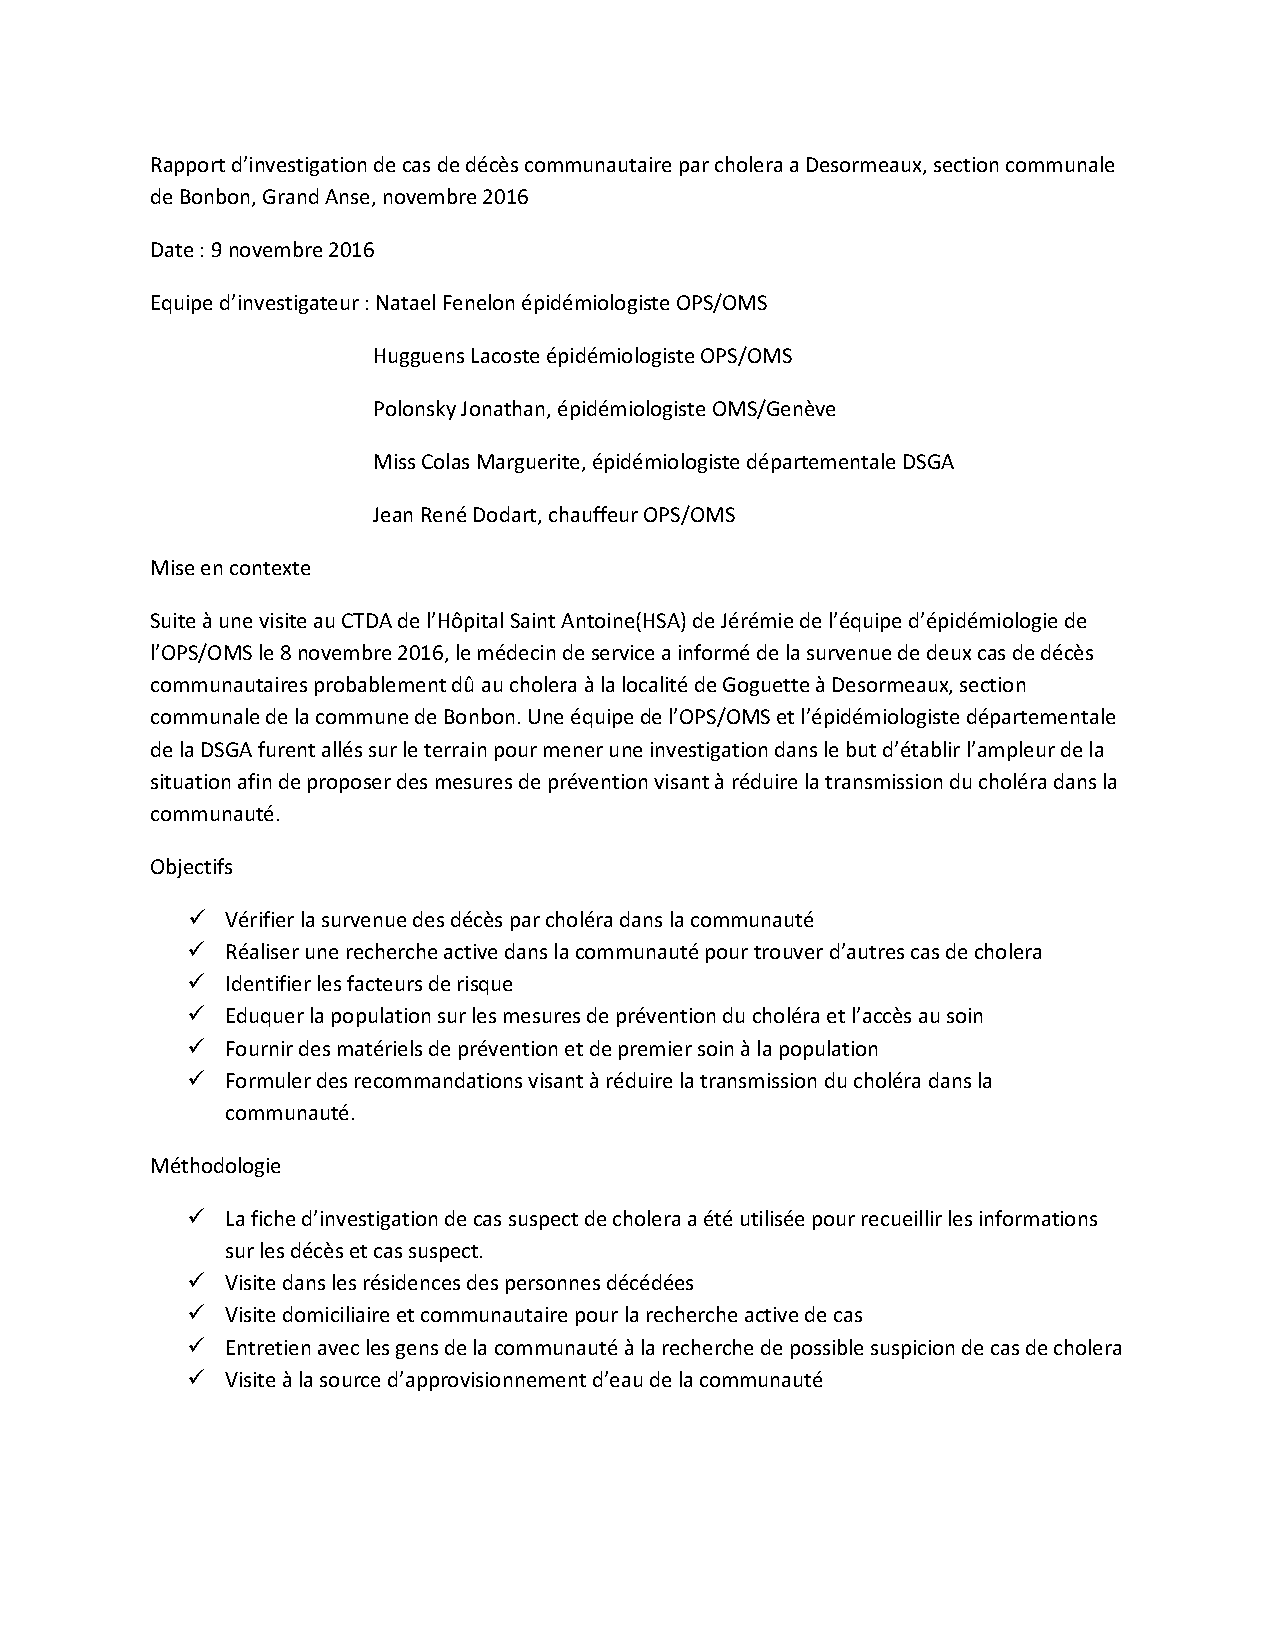
\includegraphics[page=1, width=0.8\textwidth]{annex/inv_desormeaux.pdf}
\end{figure*}

\clearpage

\begin{figure*}
\includegraphics[page=2, width=0.8\textwidth]{annex/inv_desormeaux.pdf}
\end{figure*}

\clearpage

\begin{figure*}
\includegraphics[page=3, width=0.8\textwidth]{annex/inv_desormeaux.pdf}
\end{figure*}

\clearpage

\subsection{Annex 2 - Rapport d'investigation de la flambée du choléra,
Gond'ayer,
Grand'Anse}\label{annex-2---rapport-dinvestigation-de-la-flambee-du-cholera-gondayer-grandanse}

\begin{figure*}
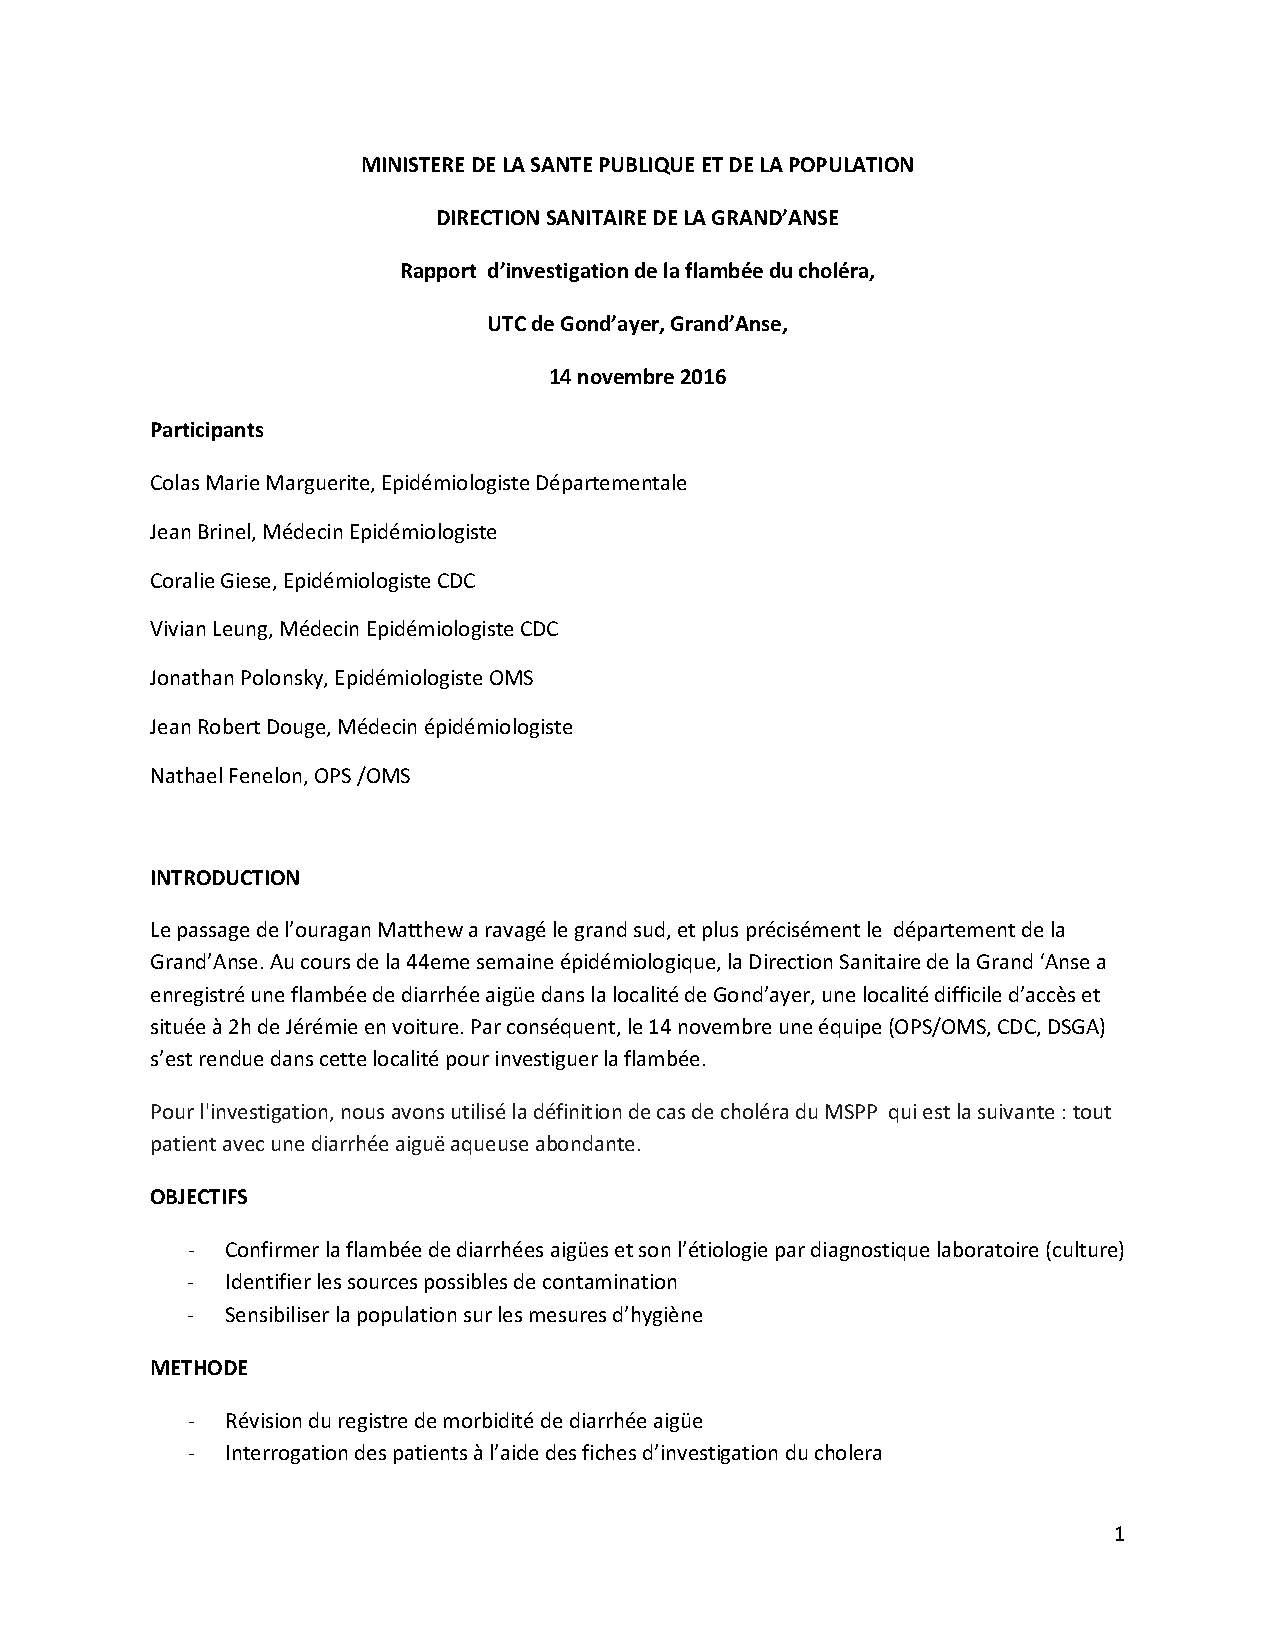
\includegraphics[page=1, width=0.8\textwidth]{annex/inv_gond_ayer.pdf}
\end{figure*}

\clearpage

\begin{figure*}
\includegraphics[page=2, width=0.8\textwidth]{annex/inv_gond_ayer.pdf}
\end{figure*}

\clearpage

\begin{figure*}
\includegraphics[page=3, width=0.8\textwidth]{annex/inv_gond_ayer.pdf}
\end{figure*}

\clearpage

\begin{figure*}
\includegraphics[page=4, width=0.8\textwidth]{annex/inv_gond_ayer.pdf}
\end{figure*}

\clearpage

\begin{figure*}
\includegraphics[page=5, width=0.8\textwidth]{annex/inv_gond_ayer.pdf}
\end{figure*}

\clearpage

\begin{figure*}
\includegraphics[page=6, width=0.8\textwidth]{annex/inv_gond_ayer.pdf}
\end{figure*}

\clearpage

\subsection{Annex 3 - Protocole d'investigation d'une flambée de
cholera}\label{annex-3---protocole-dinvestigation-dune-flambee-de-cholera}

\begin{figure*}
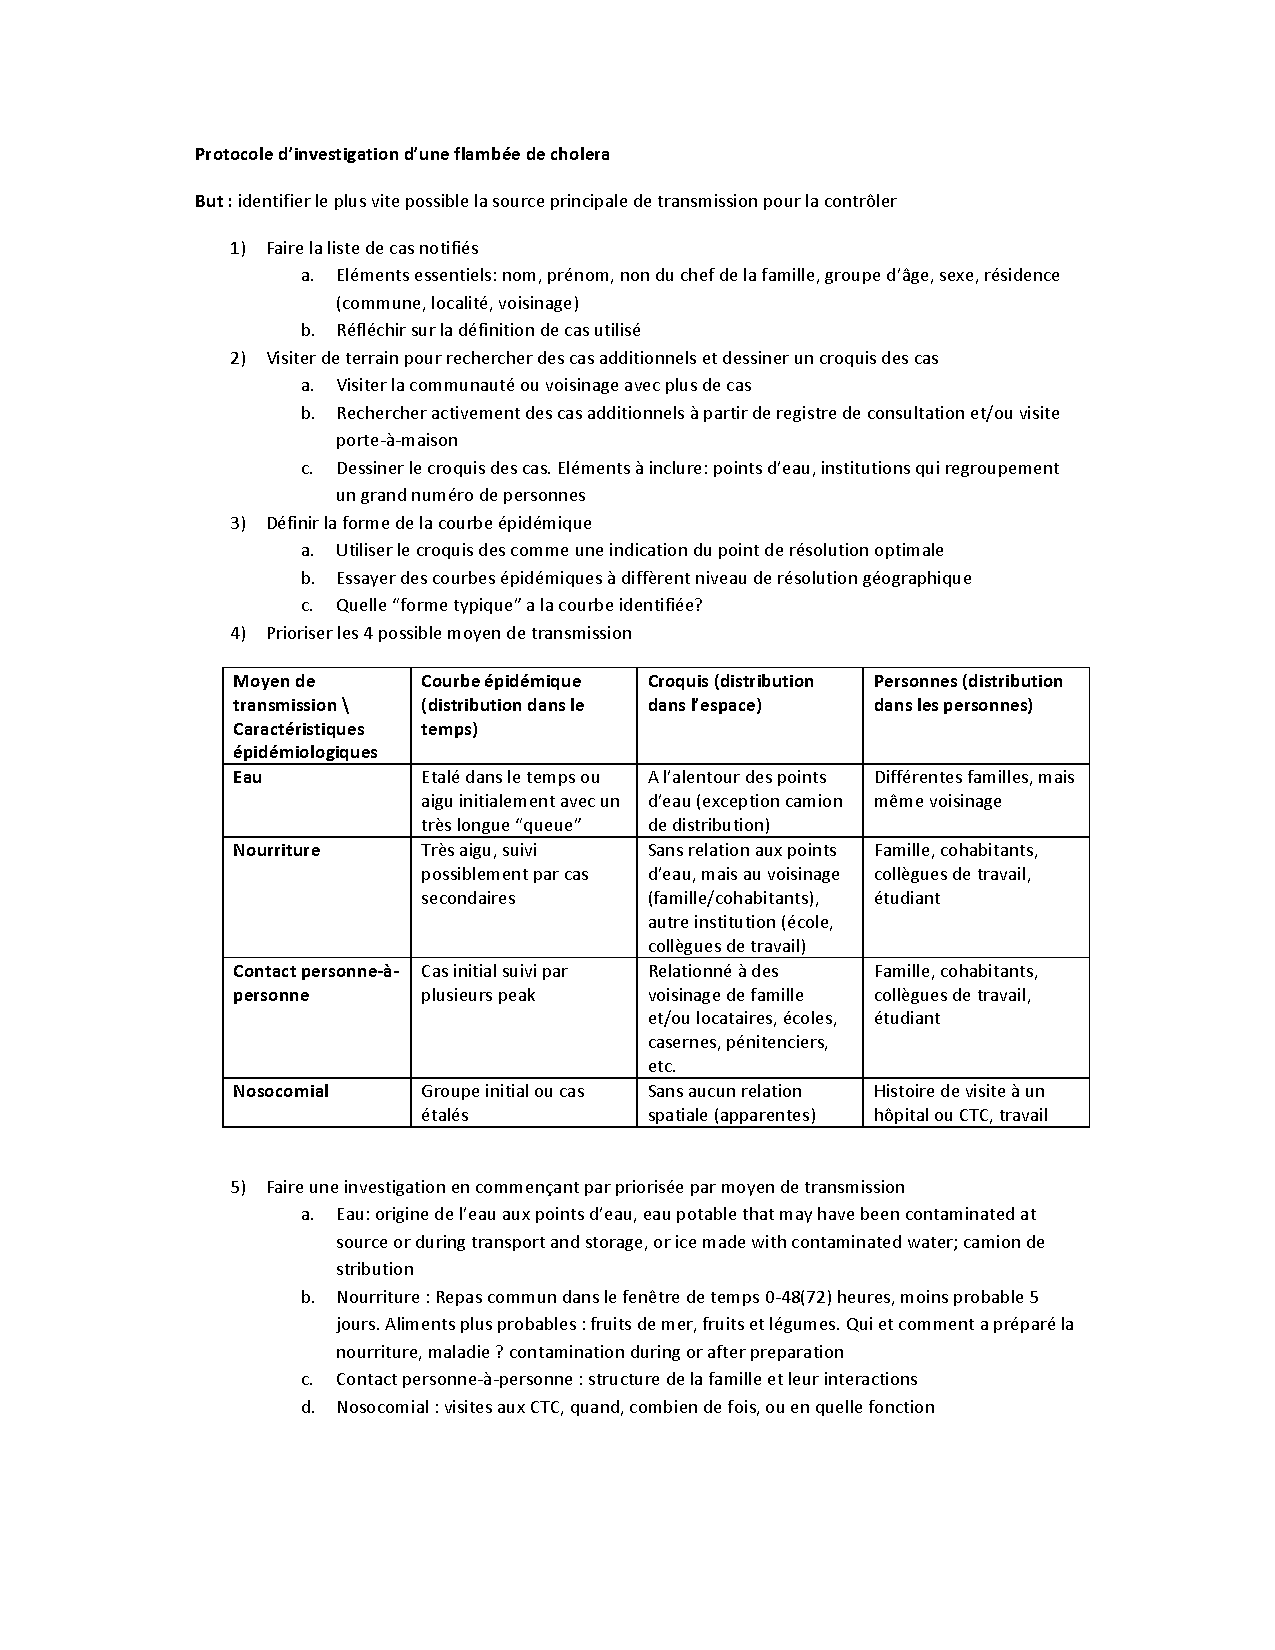
\includegraphics[width=0.8\textwidth]{annex/inv_protocole.pdf}
\end{figure*}

\clearpage

\renewcommand\refname{References}
\bibliography{refs.bib}



\end{document}
